\documentclass[1p]{elsarticle_modified}
%\bibliographystyle{elsarticle-num}

%\usepackage[colorlinks]{hyperref}
%\usepackage{abbrmath_seonhwa} %\Abb, \Ascr, \Acal ,\Abf, \Afrak
\usepackage{amsfonts}
\usepackage{amssymb}
\usepackage{amsmath}
\usepackage{amsthm}
\usepackage{scalefnt}
\usepackage{amsbsy}
\usepackage{kotex}
\usepackage{caption}
\usepackage{subfig}
\usepackage{color}
\usepackage{graphicx}
\usepackage{xcolor} %% white, black, red, green, blue, cyan, magenta, yellow
\usepackage{float}
\usepackage{setspace}
\usepackage{hyperref}

\usepackage{tikz}
\usetikzlibrary{arrows}

\usepackage{multirow}
\usepackage{array} % fixed length table
\usepackage{hhline}

%%%%%%%%%%%%%%%%%%%%%
\makeatletter
\renewcommand*\env@matrix[1][\arraystretch]{%
	\edef\arraystretch{#1}%
	\hskip -\arraycolsep
	\let\@ifnextchar\new@ifnextchar
	\array{*\c@MaxMatrixCols c}}
\makeatother %https://tex.stackexchange.com/questions/14071/how-can-i-increase-the-line-spacing-in-a-matrix
%%%%%%%%%%%%%%%

\usepackage[normalem]{ulem}

\newcommand{\msout}[1]{\ifmmode\text{\sout{\ensuremath{#1}}}\else\sout{#1}\fi}
%SOURCE: \msout is \stkout macro in https://tex.stackexchange.com/questions/20609/strikeout-in-math-mode

\newcommand{\cancel}[1]{
	\ifmmode
	{\color{red}\msout{#1}}
	\else
	{\color{red}\sout{#1}}
	\fi
}

\newcommand{\add}[1]{
	{\color{blue}\uwave{#1}}
}

\newcommand{\replace}[2]{
	\ifmmode
	{\color{red}\msout{#1}}{\color{blue}\uwave{#2}}
	\else
	{\color{red}\sout{#1}}{\color{blue}\uwave{#2}}
	\fi
}

\newcommand{\Sol}{\mathcal{S}} %segment
\newcommand{\D}{D} %diagram
\newcommand{\A}{\mathcal{A}} %arc


%%%%%%%%%%%%%%%%%%%%%%%%%%%%%5 test

\def\sl{\operatorname{\textup{SL}}(2,\Cbb)}
\def\psl{\operatorname{\textup{PSL}}(2,\Cbb)}
\def\quan{\mkern 1mu \triangleright \mkern 1mu}

\theoremstyle{definition}
\newtheorem{thm}{Theorem}[section]
\newtheorem{prop}[thm]{Proposition}
\newtheorem{lem}[thm]{Lemma}
\newtheorem{ques}[thm]{Question}
\newtheorem{cor}[thm]{Corollary}
\newtheorem{defn}[thm]{Definition}
\newtheorem{exam}[thm]{Example}
\newtheorem{rmk}[thm]{Remark}
\newtheorem{alg}[thm]{Algorithm}

\newcommand{\I}{\sqrt{-1}}
\begin{document}

%\begin{frontmatter}
%
%\title{Boundary parabolic representations of knots up to 8 crossings}
%
%%% Group authors per affiliation:
%\author{Yunhi Cho} 
%\address{Department of Mathematics, University of Seoul, Seoul, Korea}
%\ead{yhcho@uos.ac.kr}
%
%
%\author{Seonhwa Kim} %\fnref{s_kim}}
%\address{Center for Geometry and Physics, Institute for Basic Science, Pohang, 37673, Korea}
%\ead{ryeona17@ibs.re.kr}
%
%\author{Hyuk Kim}
%\address{Department of Mathematical Sciences, Seoul National University, Seoul 08826, Korea}
%\ead{hyukkim@snu.ac.kr}
%
%\author{Seokbeom Yoon}
%\address{Department of Mathematical Sciences, Seoul National University, Seoul, 08826,  Korea}
%\ead{sbyoon15@snu.ac.kr}
%
%\begin{abstract}
%We find all boundary parabolic representation of knots up to 8 crossings.
%
%\end{abstract}
%\begin{keyword}
%    \MSC[2010] 57M25 
%\end{keyword}
%
%\end{frontmatter}

%\linenumbers
%\tableofcontents
%
\newcommand\colored[1]{\textcolor{white}{\rule[-0.35ex]{0.8em}{1.4ex}}\kern-0.8em\color{red} #1}%
%\newcommand\colored[1]{\textcolor{white}{ #1}\kern-2.17ex	\textcolor{white}{ #1}\kern-1.81ex	\textcolor{white}{ #1}\kern-2.15ex\color{red}#1	}

{\Large $\underline{12a_{1052}~(K12a_{1052})}$}

\setlength{\tabcolsep}{10pt}
\renewcommand{\arraystretch}{1.6}
\vspace{1cm}\begin{tabular}{m{100pt}>{\centering\arraybackslash}m{274pt}}
\multirow{5}{120pt}{
	\centering
	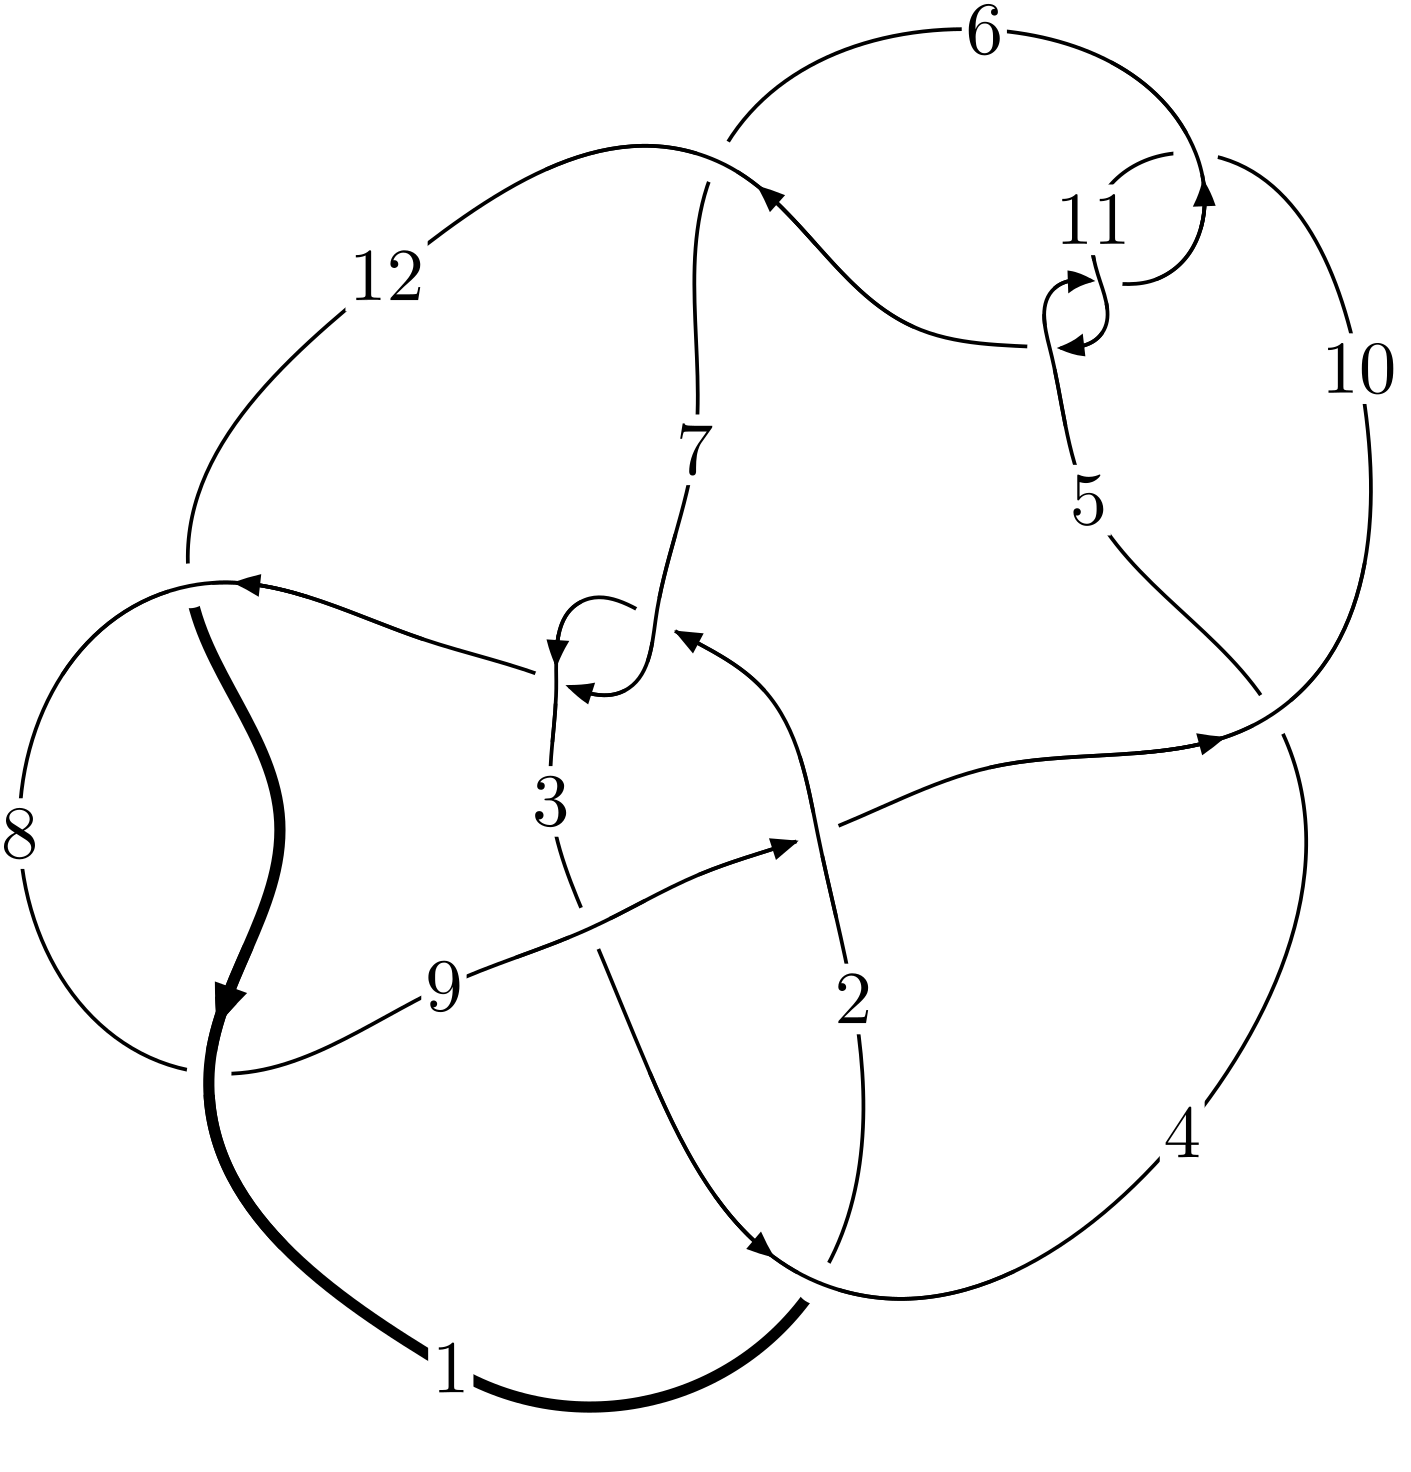
\includegraphics[width=112pt]{../../../GIT/diagram.site/Diagrams/png/1853_12a_1052.png}\\
\ \ \ A knot diagram\footnotemark}&
\allowdisplaybreaks
\textbf{Linearized knot diagam} \\
\cline{2-2}
 &
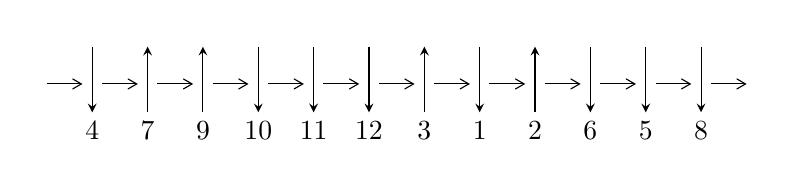
\begin{tikzpicture}[x=20pt, y=17pt]
	% nodes
	\node (C0) at (0, 0) {};
	\node (C1) at (1, 0) {};
	\node (C1U) at (1, +1) {};
	\node (C1D) at (1, -1) {4};

	\node (C2) at (2, 0) {};
	\node (C2U) at (2, +1) {};
	\node (C2D) at (2, -1) {7};

	\node (C3) at (3, 0) {};
	\node (C3U) at (3, +1) {};
	\node (C3D) at (3, -1) {9};

	\node (C4) at (4, 0) {};
	\node (C4U) at (4, +1) {};
	\node (C4D) at (4, -1) {10};

	\node (C5) at (5, 0) {};
	\node (C5U) at (5, +1) {};
	\node (C5D) at (5, -1) {11};

	\node (C6) at (6, 0) {};
	\node (C6U) at (6, +1) {};
	\node (C6D) at (6, -1) {12};

	\node (C7) at (7, 0) {};
	\node (C7U) at (7, +1) {};
	\node (C7D) at (7, -1) {3};

	\node (C8) at (8, 0) {};
	\node (C8U) at (8, +1) {};
	\node (C8D) at (8, -1) {1};

	\node (C9) at (9, 0) {};
	\node (C9U) at (9, +1) {};
	\node (C9D) at (9, -1) {2};

	\node (C10) at (10, 0) {};
	\node (C10U) at (10, +1) {};
	\node (C10D) at (10, -1) {6};

	\node (C11) at (11, 0) {};
	\node (C11U) at (11, +1) {};
	\node (C11D) at (11, -1) {5};

	\node (C12) at (12, 0) {};
	\node (C12U) at (12, +1) {};
	\node (C12D) at (12, -1) {8};
	\node (C13) at (13, 0) {};

	% arrows
	\draw[->,>={angle 60}]
	(C0) edge (C1) (C1) edge (C2) (C2) edge (C3) (C3) edge (C4) (C4) edge (C5) (C5) edge (C6) (C6) edge (C7) (C7) edge (C8) (C8) edge (C9) (C9) edge (C10) (C10) edge (C11) (C11) edge (C12) (C12) edge (C13) ;	\draw[->,>=stealth]
	(C1U) edge (C1D) (C2D) edge (C2U) (C3D) edge (C3U) (C4U) edge (C4D) (C5U) edge (C5D) (C6U) edge (C6D) (C7D) edge (C7U) (C8U) edge (C8D) (C9D) edge (C9U) (C10U) edge (C10D) (C11U) edge (C11D) (C12U) edge (C12D) ;
	\end{tikzpicture} \\
\hhline{~~} \\& 
\textbf{Solving Sequence} \\ \cline{2-2} 
 &
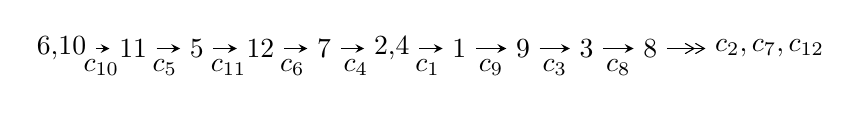
\begin{tikzpicture}[x=23pt, y=7pt]
	% node
	\node (A0) at (-1/8, 0) {6,10};
	\node (A1) at (1, 0) {11};
	\node (A2) at (2, 0) {5};
	\node (A3) at (3, 0) {12};
	\node (A4) at (4, 0) {7};
	\node (A5) at (81/16, 0) {2,4};
	\node (A6) at (49/8, 0) {1};
	\node (A7) at (57/8, 0) {9};
	\node (A8) at (65/8, 0) {3};
	\node (A9) at (73/8, 0) {8};
	\node (C1) at (1/2, -1) {$c_{10}$};
	\node (C2) at (3/2, -1) {$c_{5}$};
	\node (C3) at (5/2, -1) {$c_{11}$};
	\node (C4) at (7/2, -1) {$c_{6}$};
	\node (C5) at (9/2, -1) {$c_{4}$};
	\node (C6) at (45/8, -1) {$c_{1}$};
	\node (C7) at (53/8, -1) {$c_{9}$};
	\node (C8) at (61/8, -1) {$c_{3}$};
	\node (C9) at (69/8, -1) {$c_{8}$};
	\node (A10) at (11, 0) {$c_{2},c_{7},c_{12}$};

	% edge
	\draw[->,>=stealth]	
	(A0) edge (A1) (A1) edge (A2) (A2) edge (A3) (A3) edge (A4) (A4) edge (A5) (A5) edge (A6) (A6) edge (A7) (A7) edge (A8) (A8) edge (A9) ;
	\draw[->>,>={angle 60}]	
	(A9) edge (A10);
\end{tikzpicture} \\ 

\end{tabular} \\

\footnotetext{
The image of knot diagram is generated by the software ``\textbf{Draw programme}" developed by Andrew Bartholomew(\url{http://www.layer8.co.uk/maths/draw/index.htm\#Running-draw}), where we modified some parts for our purpose(\url{https://github.com/CATsTAILs/LinksPainter}).
}\phantom \\ \newline 
\centering \textbf{Ideals for irreducible components\footnotemark of $X_{\text{par}}$} 
 
\begin{align*}
I^u_{1}&=\langle 
7.32033\times10^{90} u^{113}-1.93522\times10^{90} u^{112}+\cdots+6.70656\times10^{90} b+1.59902\times10^{90},\\
\phantom{I^u_{1}}&\phantom{= \langle  }3.53856\times10^{91} u^{113}-2.33564\times10^{91} u^{112}+\cdots+6.70656\times10^{90} a+2.28699\times10^{92},\;u^{114}- u^{113}+\cdots+17 u-1\rangle \\
I^u_{2}&=\langle 
u^{20}+9 u^{18}+\cdots+6 u^2+b,\;u^{19}+u^{18}+\cdots+a+1,\;u^{21}+10 u^{19}+\cdots+3 u^2-1\rangle \\
\\
\end{align*}
\raggedright * 2 irreducible components of $\dim_{\mathbb{C}}=0$, with total 135 representations.\\
\footnotetext{All coefficients of polynomials are rational numbers. But the coefficients are sometimes approximated in decimal forms when there is not enough margin.}
\newpage
\renewcommand{\arraystretch}{1}
\centering \section*{I. $I^u_{1}= \langle 7.32\times10^{90} u^{113}-1.94\times10^{90} u^{112}+\cdots+6.71\times10^{90} b+1.60\times10^{90},\;3.54\times10^{91} u^{113}-2.34\times10^{91} u^{112}+\cdots+6.71\times10^{90} a+2.29\times10^{92},\;u^{114}- u^{113}+\cdots+17 u-1 \rangle$}
\flushleft \textbf{(i) Arc colorings}\\
\begin{tabular}{m{7pt} m{180pt} m{7pt} m{180pt} }
\flushright $a_{6}=$&$\begin{pmatrix}0\\u\end{pmatrix}$ \\
\flushright $a_{10}=$&$\begin{pmatrix}1\\0\end{pmatrix}$ \\
\flushright $a_{11}=$&$\begin{pmatrix}1\\u^2\end{pmatrix}$ \\
\flushright $a_{5}=$&$\begin{pmatrix}u\\u^3+u\end{pmatrix}$ \\
\flushright $a_{12}=$&$\begin{pmatrix}u^2+1\\u^4+2 u^2\end{pmatrix}$ \\
\flushright $a_{7}=$&$\begin{pmatrix}- u^5-2 u^3- u\\- u^7-3 u^5-2 u^3+u\end{pmatrix}$ \\
\flushright $a_{2}=$&$\begin{pmatrix}-5.27627 u^{113}+3.48262 u^{112}+\cdots+314.505 u-34.1008\\-1.09152 u^{113}+0.288557 u^{112}+\cdots-2.59648 u-0.238427\end{pmatrix}$ \\
\flushright $a_{4}=$&$\begin{pmatrix}u^3+2 u\\u^3+u\end{pmatrix}$ \\
\flushright $a_{1}=$&$\begin{pmatrix}-4.61041 u^{113}+3.67810 u^{112}+\cdots+314.574 u-33.6140\\-1.20888 u^{113}-0.656988 u^{112}+\cdots-18.5266 u+0.967100\end{pmatrix}$ \\
\flushright $a_{9}=$&$\begin{pmatrix}4.25189 u^{113}-5.29865 u^{112}+\cdots-335.802 u+36.0515\\-1.87637 u^{113}+2.53372 u^{112}+\cdots-19.8731 u+1.91709\end{pmatrix}$ \\
\flushright $a_{3}=$&$\begin{pmatrix}-4.87644 u^{113}+4.31876 u^{112}+\cdots+334.488 u-35.6095\\-1.22567 u^{113}-0.772076 u^{112}+\cdots-22.9954 u+1.24478\end{pmatrix}$ \\
\flushright $a_{8}=$&$\begin{pmatrix}4.47862 u^{113}-6.30012 u^{112}+\cdots-385.534 u+47.2150\\-0.612792 u^{113}+0.596277 u^{112}+\cdots-36.3318 u+4.07133\end{pmatrix}$\\&\end{tabular}
\flushleft \textbf{(ii) Obstruction class $= -1$}\\~\\
\flushleft \textbf{(iii) Cusp Shapes $= 3.96121 u^{113}-4.24884 u^{112}+\cdots-488.686 u+44.0315$}\\~\\
\newpage\renewcommand{\arraystretch}{1}
\flushleft \textbf{(iv) u-Polynomials at the component}\newline \\
\begin{tabular}{m{50pt}|m{274pt}}
Crossings & \hspace{64pt}u-Polynomials at each crossing \\
\hline $$\begin{aligned}c_{1}\end{aligned}$$&$\begin{aligned}
&u^{114}-13 u^{113}+\cdots-76092 u+7999
\end{aligned}$\\
\hline $$\begin{aligned}c_{2},c_{7}\end{aligned}$$&$\begin{aligned}
&u^{114}-33 u^{112}+\cdots+2 u+1
\end{aligned}$\\
\hline $$\begin{aligned}c_{3}\end{aligned}$$&$\begin{aligned}
&u^{114}- u^{113}+\cdots+7 u+1
\end{aligned}$\\
\hline $$\begin{aligned}c_{4},c_{6}\end{aligned}$$&$\begin{aligned}
&u^{114}+u^{113}+\cdots+60449 u-3737
\end{aligned}$\\
\hline $$\begin{aligned}c_{5},c_{10},c_{11}\end{aligned}$$&$\begin{aligned}
&u^{114}- u^{113}+\cdots+17 u-1
\end{aligned}$\\
\hline $$\begin{aligned}c_{8},c_{12}\end{aligned}$$&$\begin{aligned}
&u^{114}-40 u^{112}+\cdots+934 u+509
\end{aligned}$\\
\hline $$\begin{aligned}c_{9}\end{aligned}$$&$\begin{aligned}
&u^{114}+3 u^{113}+\cdots-2304 u+416
\end{aligned}$\\
\hline
\end{tabular}\\~\\
\newpage\renewcommand{\arraystretch}{1}
\flushleft \textbf{(v) Riley Polynomials at the component}\newline \\
\begin{tabular}{m{50pt}|m{274pt}}
Crossings & \hspace{64pt}Riley Polynomials at each crossing \\
\hline $$\begin{aligned}c_{1}\end{aligned}$$&$\begin{aligned}
&y^{114}-41 y^{113}+\cdots-1109681576 y+63984001
\end{aligned}$\\
\hline $$\begin{aligned}c_{2},c_{7}\end{aligned}$$&$\begin{aligned}
&y^{114}-66 y^{113}+\cdots-42 y+1
\end{aligned}$\\
\hline $$\begin{aligned}c_{3}\end{aligned}$$&$\begin{aligned}
&y^{114}+11 y^{113}+\cdots+15 y+1
\end{aligned}$\\
\hline $$\begin{aligned}c_{4},c_{6}\end{aligned}$$&$\begin{aligned}
&y^{114}-85 y^{113}+\cdots-1006282569 y+13965169
\end{aligned}$\\
\hline $$\begin{aligned}c_{5},c_{10},c_{11}\end{aligned}$$&$\begin{aligned}
&y^{114}+95 y^{113}+\cdots-89 y+1
\end{aligned}$\\
\hline $$\begin{aligned}c_{8},c_{12}\end{aligned}$$&$\begin{aligned}
&y^{114}-80 y^{113}+\cdots-10221668 y+259081
\end{aligned}$\\
\hline $$\begin{aligned}c_{9}\end{aligned}$$&$\begin{aligned}
&y^{114}+13 y^{113}+\cdots+3856896 y+173056
\end{aligned}$\\
\hline
\end{tabular}\\~\\
\newpage\flushleft \textbf{(vi) Complex Volumes and Cusp Shapes}
$$\begin{array}{c|c|c}  
\text{Solutions to }I^u_{1}& \I (\text{vol} + \sqrt{-1}CS) & \text{Cusp shape}\\
 \hline 
\begin{aligned}
u &= \phantom{-}0.887561 + 0.033463 I \\
a &= \phantom{-}0.667047 - 0.840543 I \\
b &= \phantom{-}0.761693 - 0.542709 I\end{aligned}
 & -8.87011 - 0.11224 I & \phantom{-0.000000 } 0 \\ \hline\begin{aligned}
u &= \phantom{-}0.887561 - 0.033463 I \\
a &= \phantom{-}0.667047 + 0.840543 I \\
b &= \phantom{-}0.761693 + 0.542709 I\end{aligned}
 & -8.87011 + 0.11224 I & \phantom{-0.000000 } 0 \\ \hline\begin{aligned}
u &= \phantom{-}0.884055\phantom{ +0.000000I} \\
a &= \phantom{-}1.57119\phantom{ +0.000000I} \\
b &= \phantom{-}1.32521\phantom{ +0.000000I}\end{aligned}
 & -8.83336\phantom{ +0.000000I} & \phantom{-0.000000 } 0 \\ \hline\begin{aligned}
u &= \phantom{-}0.861941 + 0.130288 I \\
a &= \phantom{-}0.66446 - 2.36238 I \\
b &= \phantom{-}1.12530 - 1.26937 I\end{aligned}
 & -6.2381 - 13.5633 I & \phantom{-0.000000 } 0 \\ \hline\begin{aligned}
u &= \phantom{-}0.861941 - 0.130288 I \\
a &= \phantom{-}0.66446 + 2.36238 I \\
b &= \phantom{-}1.12530 + 1.26937 I\end{aligned}
 & -6.2381 + 13.5633 I & \phantom{-0.000000 } 0 \\ \hline\begin{aligned}
u &= -0.855647 + 0.157410 I \\
a &= -0.36775 + 1.65160 I \\
b &= \phantom{-}0.174619 + 1.137200 I\end{aligned}
 & -6.26667 + 4.41214 I & \phantom{-0.000000 } 0 \\ \hline\begin{aligned}
u &= -0.855647 - 0.157410 I \\
a &= -0.36775 - 1.65160 I \\
b &= \phantom{-}0.174619 - 1.137200 I\end{aligned}
 & -6.26667 - 4.41214 I & \phantom{-0.000000 } 0 \\ \hline\begin{aligned}
u &= -0.420494 + 1.077840 I \\
a &= -0.472262 + 0.757702 I \\
b &= \phantom{-}0.009418 + 1.138830 I\end{aligned}
 & -3.43938 + 0.18223 I & \phantom{-0.000000 } 0 \\ \hline\begin{aligned}
u &= -0.420494 - 1.077840 I \\
a &= -0.472262 - 0.757702 I \\
b &= \phantom{-}0.009418 - 1.138830 I\end{aligned}
 & -3.43938 - 0.18223 I & \phantom{-0.000000 } 0 \\ \hline\begin{aligned}
u &= -0.838651 + 0.073965 I \\
a &= \phantom{-}0.35169 + 2.00996 I \\
b &= \phantom{-}0.986139 + 0.983905 I\end{aligned}
 & -9.16090 + 6.43907 I & \phantom{-0.000000 } 0\\
 \hline 
 \end{array}$$\newpage$$\begin{array}{c|c|c}  
\text{Solutions to }I^u_{1}& \I (\text{vol} + \sqrt{-1}CS) & \text{Cusp shape}\\
 \hline 
\begin{aligned}
u &= -0.838651 - 0.073965 I \\
a &= \phantom{-}0.35169 - 2.00996 I \\
b &= \phantom{-}0.986139 - 0.983905 I\end{aligned}
 & -9.16090 - 6.43907 I & \phantom{-0.000000 } 0 \\ \hline\begin{aligned}
u &= -0.836559 + 0.094115 I \\
a &= -1.11752 - 2.62098 I \\
b &= -1.21368 - 1.37230 I\end{aligned}
 & -2.01821 + 6.94038 I & \phantom{-0.000000 } 0 \\ \hline\begin{aligned}
u &= -0.836559 - 0.094115 I \\
a &= -1.11752 + 2.62098 I \\
b &= -1.21368 + 1.37230 I\end{aligned}
 & -2.01821 - 6.94038 I & \phantom{-0.000000 } 0 \\ \hline\begin{aligned}
u &= -0.034680 + 1.171200 I \\
a &= -1.05610 + 0.95379 I \\
b &= \phantom{-}1.114310 - 0.346505 I\end{aligned}
 & \phantom{-}1.35481 + 2.41007 I & \phantom{-0.000000 } 0 \\ \hline\begin{aligned}
u &= -0.034680 - 1.171200 I \\
a &= -1.05610 - 0.95379 I \\
b &= \phantom{-}1.114310 + 0.346505 I\end{aligned}
 & \phantom{-}1.35481 - 2.41007 I & \phantom{-0.000000 } 0 \\ \hline\begin{aligned}
u &= -0.799088 + 0.028521 I \\
a &= \phantom{-}1.61160 - 2.64644 I \\
b &= \phantom{-}1.34739 - 1.59685 I\end{aligned}
 & -5.95563 + 3.80586 I & -11.44875 - 3.61947 I \\ \hline\begin{aligned}
u &= -0.799088 - 0.028521 I \\
a &= \phantom{-}1.61160 + 2.64644 I \\
b &= \phantom{-}1.34739 + 1.59685 I\end{aligned}
 & -5.95563 - 3.80586 I & -11.44875 + 3.61947 I \\ \hline\begin{aligned}
u &= -0.631624 + 0.489717 I \\
a &= \phantom{-}0.972513 + 0.063768 I \\
b &= \phantom{-}0.544420 - 0.666919 I\end{aligned}
 & -1.07011 - 4.46542 I & \phantom{-0.000000 -}0. + 4.95137 I \\ \hline\begin{aligned}
u &= -0.631624 - 0.489717 I \\
a &= \phantom{-}0.972513 - 0.063768 I \\
b &= \phantom{-}0.544420 + 0.666919 I\end{aligned}
 & -1.07011 + 4.46542 I & \phantom{-0.000000 } 0. - 4.95137 I \\ \hline\begin{aligned}
u &= -0.194897 + 1.186990 I \\
a &= -0.384797 + 0.465226 I \\
b &= \phantom{-}0.374866 - 0.496573 I\end{aligned}
 & \phantom{-}2.30672 + 2.64556 I & \phantom{-0.000000 } 0\\
 \hline 
 \end{array}$$\newpage$$\begin{array}{c|c|c}  
\text{Solutions to }I^u_{1}& \I (\text{vol} + \sqrt{-1}CS) & \text{Cusp shape}\\
 \hline 
\begin{aligned}
u &= -0.194897 - 1.186990 I \\
a &= -0.384797 - 0.465226 I \\
b &= \phantom{-}0.374866 + 0.496573 I\end{aligned}
 & \phantom{-}2.30672 - 2.64556 I & \phantom{-0.000000 } 0 \\ \hline\begin{aligned}
u &= \phantom{-}0.302875 + 1.165030 I \\
a &= \phantom{-}0.338380 + 0.916390 I \\
b &= \phantom{-}0.332156 + 1.047030 I\end{aligned}
 & -0.924303 - 0.501252 I & \phantom{-0.000000 } 0 \\ \hline\begin{aligned}
u &= \phantom{-}0.302875 - 1.165030 I \\
a &= \phantom{-}0.338380 - 0.916390 I \\
b &= \phantom{-}0.332156 - 1.047030 I\end{aligned}
 & -0.924303 + 0.501252 I & \phantom{-0.000000 } 0 \\ \hline\begin{aligned}
u &= \phantom{-}0.433363 + 1.126810 I \\
a &= -0.937304 - 0.439869 I \\
b &= -1.00068 - 1.24442 I\end{aligned}
 & -3.18527 + 8.92336 I & \phantom{-0.000000 } 0 \\ \hline\begin{aligned}
u &= \phantom{-}0.433363 - 1.126810 I \\
a &= -0.937304 + 0.439869 I \\
b &= -1.00068 + 1.24442 I\end{aligned}
 & -3.18527 - 8.92336 I & \phantom{-0.000000 } 0 \\ \hline\begin{aligned}
u &= -0.559272 + 0.553878 I \\
a &= \phantom{-}0.046469 - 0.925572 I \\
b &= -0.781859 - 0.851553 I\end{aligned}
 & -0.82179 + 8.69014 I & -4.00000 - 9.28919 I \\ \hline\begin{aligned}
u &= -0.559272 - 0.553878 I \\
a &= \phantom{-}0.046469 + 0.925572 I \\
b &= -0.781859 + 0.851553 I\end{aligned}
 & -0.82179 - 8.69014 I & -4.00000 + 9.28919 I \\ \hline\begin{aligned}
u &= -0.772600 + 0.037228 I \\
a &= \phantom{-}0.61904 + 1.35329 I \\
b &= \phantom{-}0.011448 + 0.359945 I\end{aligned}
 & -1.70108 + 1.04212 I & -5.52078 - 1.15687 I \\ \hline\begin{aligned}
u &= -0.772600 - 0.037228 I \\
a &= \phantom{-}0.61904 - 1.35329 I \\
b &= \phantom{-}0.011448 - 0.359945 I\end{aligned}
 & -1.70108 - 1.04212 I & -5.52078 + 1.15687 I \\ \hline\begin{aligned}
u &= \phantom{-}0.764051 + 0.115411 I \\
a &= \phantom{-}0.31036 + 2.12630 I \\
b &= -0.446089 + 1.030000 I\end{aligned}
 & -4.09501 - 3.38991 I & -10.58127 + 2.23573 I\\
 \hline 
 \end{array}$$\newpage$$\begin{array}{c|c|c}  
\text{Solutions to }I^u_{1}& \I (\text{vol} + \sqrt{-1}CS) & \text{Cusp shape}\\
 \hline 
\begin{aligned}
u &= \phantom{-}0.764051 - 0.115411 I \\
a &= \phantom{-}0.31036 - 2.12630 I \\
b &= -0.446089 - 1.030000 I\end{aligned}
 & -4.09501 + 3.38991 I & -10.58127 - 2.23573 I \\ \hline\begin{aligned}
u &= \phantom{-}0.769870\phantom{ +0.000000I} \\
a &= \phantom{-}0.648054\phantom{ +0.000000I} \\
b &= \phantom{-}1.32831\phantom{ +0.000000I}\end{aligned}
 & -0.697644\phantom{ +0.000000I} & -8.68980\phantom{ +0.000000I} \\ \hline\begin{aligned}
u &= \phantom{-}0.762064 + 0.089577 I \\
a &= -0.30317 + 2.09043 I \\
b &= -0.339727 + 0.412420 I\end{aligned}
 & -2.72396 - 5.39723 I & -4.97222 + 8.97168 I \\ \hline\begin{aligned}
u &= \phantom{-}0.762064 - 0.089577 I \\
a &= -0.30317 - 2.09043 I \\
b &= -0.339727 - 0.412420 I\end{aligned}
 & -2.72396 + 5.39723 I & -4.97222 - 8.97168 I \\ \hline\begin{aligned}
u &= -0.385495 + 1.171350 I \\
a &= \phantom{-}1.341730 - 0.444799 I \\
b &= \phantom{-}1.04075 - 1.34482 I\end{aligned}
 & \phantom{-}1.28099 - 2.53613 I & \phantom{-0.000000 } 0 \\ \hline\begin{aligned}
u &= -0.385495 - 1.171350 I \\
a &= \phantom{-}1.341730 + 0.444799 I \\
b &= \phantom{-}1.04075 + 1.34482 I\end{aligned}
 & \phantom{-}1.28099 + 2.53613 I & \phantom{-0.000000 } 0 \\ \hline\begin{aligned}
u &= \phantom{-}0.283143 + 1.201940 I \\
a &= \phantom{-}0.55050 + 1.52618 I \\
b &= \phantom{-}0.168272 + 0.232893 I\end{aligned}
 & \phantom{-}0.62179 + 1.60000 I & \phantom{-0.000000 } 0 \\ \hline\begin{aligned}
u &= \phantom{-}0.283143 - 1.201940 I \\
a &= \phantom{-}0.55050 - 1.52618 I \\
b &= \phantom{-}0.168272 - 0.232893 I\end{aligned}
 & \phantom{-}0.62179 - 1.60000 I & \phantom{-0.000000 } 0 \\ \hline\begin{aligned}
u &= \phantom{-}0.756287 + 0.034907 I \\
a &= -0.01534 + 2.83346 I \\
b &= -0.55058 + 1.35141 I\end{aligned}
 & -4.02624 - 3.05369 I & -8.42676 + 2.90164 I \\ \hline\begin{aligned}
u &= \phantom{-}0.756287 - 0.034907 I \\
a &= -0.01534 - 2.83346 I \\
b &= -0.55058 - 1.35141 I\end{aligned}
 & -4.02624 + 3.05369 I & -8.42676 - 2.90164 I\\
 \hline 
 \end{array}$$\newpage$$\begin{array}{c|c|c}  
\text{Solutions to }I^u_{1}& \I (\text{vol} + \sqrt{-1}CS) & \text{Cusp shape}\\
 \hline 
\begin{aligned}
u &= \phantom{-}0.368655 + 0.653613 I \\
a &= \phantom{-}0.362791 + 0.342465 I \\
b &= \phantom{-}0.315800 + 0.964205 I\end{aligned}
 & -2.18652 + 0.53327 I & -7.37777 + 1.33068 I \\ \hline\begin{aligned}
u &= \phantom{-}0.368655 - 0.653613 I \\
a &= \phantom{-}0.362791 - 0.342465 I \\
b &= \phantom{-}0.315800 - 0.964205 I\end{aligned}
 & -2.18652 - 0.53327 I & -7.37777 - 1.33068 I \\ \hline\begin{aligned}
u &= -0.389371 + 1.194790 I \\
a &= -0.417451 + 0.445391 I \\
b &= -0.900074 + 1.060790 I\end{aligned}
 & -5.71894 - 2.02281 I & \phantom{-0.000000 } 0 \\ \hline\begin{aligned}
u &= -0.389371 - 1.194790 I \\
a &= -0.417451 - 0.445391 I \\
b &= -0.900074 - 1.060790 I\end{aligned}
 & -5.71894 + 2.02281 I & \phantom{-0.000000 } 0 \\ \hline\begin{aligned}
u &= -0.312733 + 1.245960 I \\
a &= -0.788461 + 0.880942 I \\
b &= \phantom{-}0.226218 + 0.195802 I\end{aligned}
 & \phantom{-}2.01023 + 2.87194 I & \phantom{-0.000000 } 0 \\ \hline\begin{aligned}
u &= -0.312733 - 1.245960 I \\
a &= -0.788461 - 0.880942 I \\
b &= \phantom{-}0.226218 - 0.195802 I\end{aligned}
 & \phantom{-}2.01023 - 2.87194 I & \phantom{-0.000000 } 0 \\ \hline\begin{aligned}
u &= \phantom{-}0.033169 + 1.286540 I \\
a &= -0.475286 + 0.111459 I \\
b &= \phantom{-}0.45164 + 1.73582 I\end{aligned}
 & \phantom{-}2.83720 - 3.54184 I & \phantom{-0.000000 } 0 \\ \hline\begin{aligned}
u &= \phantom{-}0.033169 - 1.286540 I \\
a &= -0.475286 - 0.111459 I \\
b &= \phantom{-}0.45164 - 1.73582 I\end{aligned}
 & \phantom{-}2.83720 + 3.54184 I & \phantom{-0.000000 } 0 \\ \hline\begin{aligned}
u &= \phantom{-}0.019067 + 1.288260 I \\
a &= -0.86674 - 1.65349 I \\
b &= \phantom{-}0.859718 - 0.367698 I\end{aligned}
 & \phantom{-}6.84727 - 0.41254 I & \phantom{-0.000000 } 0 \\ \hline\begin{aligned}
u &= \phantom{-}0.019067 - 1.288260 I \\
a &= -0.86674 + 1.65349 I \\
b &= \phantom{-}0.859718 + 0.367698 I\end{aligned}
 & \phantom{-}6.84727 + 0.41254 I & \phantom{-0.000000 } 0\\
 \hline 
 \end{array}$$\newpage$$\begin{array}{c|c|c}  
\text{Solutions to }I^u_{1}& \I (\text{vol} + \sqrt{-1}CS) & \text{Cusp shape}\\
 \hline 
\begin{aligned}
u &= -0.348064 + 1.245640 I \\
a &= \phantom{-}1.07973 - 2.09369 I \\
b &= -1.44236 - 1.42499 I\end{aligned}
 & -2.19698 + 0.32673 I & \phantom{-0.000000 } 0 \\ \hline\begin{aligned}
u &= -0.348064 - 1.245640 I \\
a &= \phantom{-}1.07973 + 2.09369 I \\
b &= -1.44236 + 1.42499 I\end{aligned}
 & -2.19698 - 0.32673 I & \phantom{-0.000000 } 0 \\ \hline\begin{aligned}
u &= \phantom{-}0.314287 + 1.257980 I \\
a &= \phantom{-}0.98429 + 1.16072 I \\
b &= \phantom{-}0.39966 + 1.57679 I\end{aligned}
 & -0.241377 - 0.796662 I & \phantom{-0.000000 } 0 \\ \hline\begin{aligned}
u &= \phantom{-}0.314287 - 1.257980 I \\
a &= \phantom{-}0.98429 - 1.16072 I \\
b &= \phantom{-}0.39966 - 1.57679 I\end{aligned}
 & -0.241377 + 0.796662 I & \phantom{-0.000000 } 0 \\ \hline\begin{aligned}
u &= \phantom{-}0.446966 + 1.234100 I \\
a &= -0.288788 - 0.032285 I \\
b &= -0.433345 - 0.625329 I\end{aligned}
 & -5.16161 - 4.65132 I & \phantom{-0.000000 } 0 \\ \hline\begin{aligned}
u &= \phantom{-}0.446966 - 1.234100 I \\
a &= -0.288788 + 0.032285 I \\
b &= -0.433345 + 0.625329 I\end{aligned}
 & -5.16161 + 4.65132 I & \phantom{-0.000000 } 0 \\ \hline\begin{aligned}
u &= \phantom{-}0.329032 + 1.273180 I \\
a &= \phantom{-}0.672769 + 0.766233 I \\
b &= -1.335070 - 0.128239 I\end{aligned}
 & \phantom{-}3.25821 - 3.96182 I & \phantom{-0.000000 } 0 \\ \hline\begin{aligned}
u &= \phantom{-}0.329032 - 1.273180 I \\
a &= \phantom{-}0.672769 - 0.766233 I \\
b &= -1.335070 + 0.128239 I\end{aligned}
 & \phantom{-}3.25821 + 3.96182 I & \phantom{-0.000000 } 0 \\ \hline\begin{aligned}
u &= \phantom{-}0.118691 + 1.310740 I \\
a &= -1.86300 + 0.21647 I \\
b &= \phantom{-}0.590937 - 0.530944 I\end{aligned}
 & \phantom{-}1.60694 - 5.76070 I & \phantom{-0.000000 } 0 \\ \hline\begin{aligned}
u &= \phantom{-}0.118691 - 1.310740 I \\
a &= -1.86300 - 0.21647 I \\
b &= \phantom{-}0.590937 + 0.530944 I\end{aligned}
 & \phantom{-}1.60694 + 5.76070 I & \phantom{-0.000000 } 0\\
 \hline 
 \end{array}$$\newpage$$\begin{array}{c|c|c}  
\text{Solutions to }I^u_{1}& \I (\text{vol} + \sqrt{-1}CS) & \text{Cusp shape}\\
 \hline 
\begin{aligned}
u &= -0.040353 + 1.316630 I \\
a &= \phantom{-}1.193600 + 0.254814 I \\
b &= -0.664084 - 0.488787 I\end{aligned}
 & \phantom{-}4.67481 + 1.79142 I & \phantom{-0.000000 } 0 \\ \hline\begin{aligned}
u &= -0.040353 - 1.316630 I \\
a &= \phantom{-}1.193600 - 0.254814 I \\
b &= -0.664084 + 0.488787 I\end{aligned}
 & \phantom{-}4.67481 - 1.79142 I & \phantom{-0.000000 } 0 \\ \hline\begin{aligned}
u &= -0.350707 + 1.289720 I \\
a &= -1.49684 + 0.06917 I \\
b &= -1.26736 + 1.75060 I\end{aligned}
 & -1.84646 + 7.94723 I & \phantom{-0.000000 } 0 \\ \hline\begin{aligned}
u &= -0.350707 - 1.289720 I \\
a &= -1.49684 - 0.06917 I \\
b &= -1.26736 - 1.75060 I\end{aligned}
 & -1.84646 - 7.94723 I & \phantom{-0.000000 } 0 \\ \hline\begin{aligned}
u &= -0.336746 + 1.293450 I \\
a &= -0.125394 - 1.215930 I \\
b &= -0.148005 - 0.510473 I\end{aligned}
 & \phantom{-}2.45095 + 5.04973 I & \phantom{-0.000000 } 0 \\ \hline\begin{aligned}
u &= -0.336746 - 1.293450 I \\
a &= -0.125394 + 1.215930 I \\
b &= -0.148005 + 0.510473 I\end{aligned}
 & \phantom{-}2.45095 - 5.04973 I & \phantom{-0.000000 } 0 \\ \hline\begin{aligned}
u &= \phantom{-}0.329752 + 1.298790 I \\
a &= -1.46795 - 1.54358 I \\
b &= \phantom{-}0.74460 - 1.22192 I\end{aligned}
 & \phantom{-}0.15037 - 6.98175 I & \phantom{-0.000000 } 0 \\ \hline\begin{aligned}
u &= \phantom{-}0.329752 - 1.298790 I \\
a &= -1.46795 + 1.54358 I \\
b &= \phantom{-}0.74460 + 1.22192 I\end{aligned}
 & \phantom{-}0.15037 + 6.98175 I & \phantom{-0.000000 } 0 \\ \hline\begin{aligned}
u &= \phantom{-}0.417386 + 1.276610 I \\
a &= -0.557000 + 0.889935 I \\
b &= -1.338270 - 0.222985 I\end{aligned}
 & -4.86969 - 4.65741 I & \phantom{-0.000000 } 0 \\ \hline\begin{aligned}
u &= \phantom{-}0.417386 - 1.276610 I \\
a &= -0.557000 - 0.889935 I \\
b &= -1.338270 + 0.222985 I\end{aligned}
 & -4.86969 + 4.65741 I & \phantom{-0.000000 } 0\\
 \hline 
 \end{array}$$\newpage$$\begin{array}{c|c|c}  
\text{Solutions to }I^u_{1}& \I (\text{vol} + \sqrt{-1}CS) & \text{Cusp shape}\\
 \hline 
\begin{aligned}
u &= -0.274471 + 1.318860 I \\
a &= -0.644135 + 0.621966 I \\
b &= \phantom{-}1.059720 - 0.139345 I\end{aligned}
 & \phantom{-}3.34166 + 3.14281 I & \phantom{-0.000000 } 0 \\ \hline\begin{aligned}
u &= -0.274471 - 1.318860 I \\
a &= -0.644135 - 0.621966 I \\
b &= \phantom{-}1.059720 + 0.139345 I\end{aligned}
 & \phantom{-}3.34166 - 3.14281 I & \phantom{-0.000000 } 0 \\ \hline\begin{aligned}
u &= \phantom{-}0.405592 + 1.294220 I \\
a &= \phantom{-}0.256254 + 1.094430 I \\
b &= -1.014100 + 0.529729 I\end{aligned}
 & -4.73797 - 4.73329 I & \phantom{-0.000000 } 0 \\ \hline\begin{aligned}
u &= \phantom{-}0.405592 - 1.294220 I \\
a &= \phantom{-}0.256254 - 1.094430 I \\
b &= -1.014100 - 0.529729 I\end{aligned}
 & -4.73797 + 4.73329 I & \phantom{-0.000000 } 0 \\ \hline\begin{aligned}
u &= \phantom{-}0.180288 + 1.348920 I \\
a &= \phantom{-}0.047717 - 1.084830 I \\
b &= \phantom{-}1.069820 + 0.119273 I\end{aligned}
 & \phantom{-}8.05571 - 1.71787 I & \phantom{-0.000000 } 0 \\ \hline\begin{aligned}
u &= \phantom{-}0.180288 - 1.348920 I \\
a &= \phantom{-}0.047717 + 1.084830 I \\
b &= \phantom{-}1.069820 - 0.119273 I\end{aligned}
 & \phantom{-}8.05571 + 1.71787 I & \phantom{-0.000000 } 0 \\ \hline\begin{aligned}
u &= -0.030908 + 1.363840 I \\
a &= \phantom{-}1.25211 - 0.87845 I \\
b &= -0.814496 - 0.347039 I\end{aligned}
 & \phantom{-}6.34340 + 3.23650 I & \phantom{-0.000000 } 0 \\ \hline\begin{aligned}
u &= -0.030908 - 1.363840 I \\
a &= \phantom{-}1.25211 + 0.87845 I \\
b &= -0.814496 + 0.347039 I\end{aligned}
 & \phantom{-}6.34340 - 3.23650 I & \phantom{-0.000000 } 0 \\ \hline\begin{aligned}
u &= \phantom{-}0.330308 + 1.325050 I \\
a &= -0.53730 - 1.74794 I \\
b &= \phantom{-}0.419800 - 0.520125 I\end{aligned}
 & \phantom{-}1.71717 - 9.35311 I & \phantom{-0.000000 } 0 \\ \hline\begin{aligned}
u &= \phantom{-}0.330308 - 1.325050 I \\
a &= -0.53730 + 1.74794 I \\
b &= \phantom{-}0.419800 + 0.520125 I\end{aligned}
 & \phantom{-}1.71717 + 9.35311 I & \phantom{-0.000000 } 0\\
 \hline 
 \end{array}$$\newpage$$\begin{array}{c|c|c}  
\text{Solutions to }I^u_{1}& \I (\text{vol} + \sqrt{-1}CS) & \text{Cusp shape}\\
 \hline 
\begin{aligned}
u &= -0.373340 + 1.320330 I \\
a &= \phantom{-}1.21371 - 1.55752 I \\
b &= -1.042950 - 0.908818 I\end{aligned}
 & -4.79616 + 10.79540 I & \phantom{-0.000000 } 0 \\ \hline\begin{aligned}
u &= -0.373340 - 1.320330 I \\
a &= \phantom{-}1.21371 + 1.55752 I \\
b &= -1.042950 + 0.908818 I\end{aligned}
 & -4.79616 - 10.79540 I & \phantom{-0.000000 } 0 \\ \hline\begin{aligned}
u &= \phantom{-}0.108689 + 1.371010 I \\
a &= \phantom{-}1.061600 + 0.206574 I \\
b &= -1.33473 + 0.73220 I\end{aligned}
 & \phantom{-}8.86434 - 5.29938 I & \phantom{-0.000000 } 0 \\ \hline\begin{aligned}
u &= \phantom{-}0.108689 - 1.371010 I \\
a &= \phantom{-}1.061600 - 0.206574 I \\
b &= -1.33473 - 0.73220 I\end{aligned}
 & \phantom{-}8.86434 + 5.29938 I & \phantom{-0.000000 } 0 \\ \hline\begin{aligned}
u &= -0.370406 + 1.333370 I \\
a &= -0.93236 + 1.98221 I \\
b &= \phantom{-}1.33934 + 1.36558 I\end{aligned}
 & \phantom{-}2.46011 + 11.28260 I & \phantom{-0.000000 } 0 \\ \hline\begin{aligned}
u &= -0.370406 - 1.333370 I \\
a &= -0.93236 - 1.98221 I \\
b &= \phantom{-}1.33934 - 1.36558 I\end{aligned}
 & \phantom{-}2.46011 - 11.28260 I & \phantom{-0.000000 } 0 \\ \hline\begin{aligned}
u &= -0.603702 + 0.119908 I \\
a &= -0.568367 - 0.079694 I \\
b &= -0.984828 + 0.073067 I\end{aligned}
 & -1.118330 - 0.146384 I & -7.95111 - 0.77273 I \\ \hline\begin{aligned}
u &= -0.603702 - 0.119908 I \\
a &= -0.568367 + 0.079694 I \\
b &= -0.984828 - 0.073067 I\end{aligned}
 & -1.118330 + 0.146384 I & -7.95111 + 0.77273 I \\ \hline\begin{aligned}
u &= \phantom{-}0.328033 + 1.346520 I \\
a &= -1.25207 - 1.10692 I \\
b &= \phantom{-}0.527323 - 1.006500 I\end{aligned}
 & \phantom{-}0.51996 - 7.34154 I & \phantom{-0.000000 } 0 \\ \hline\begin{aligned}
u &= \phantom{-}0.328033 - 1.346520 I \\
a &= -1.25207 + 1.10692 I \\
b &= \phantom{-}0.527323 + 1.006500 I\end{aligned}
 & \phantom{-}0.51996 + 7.34154 I & \phantom{-0.000000 } 0\\
 \hline 
 \end{array}$$\newpage$$\begin{array}{c|c|c}  
\text{Solutions to }I^u_{1}& \I (\text{vol} + \sqrt{-1}CS) & \text{Cusp shape}\\
 \hline 
\begin{aligned}
u &= \phantom{-}0.416646 + 0.435532 I \\
a &= \phantom{-}0.260901 - 1.084610 I \\
b &= \phantom{-}0.979372 - 0.738723 I\end{aligned}
 & \phantom{-}3.22241 - 3.59528 I & \phantom{-}0.10104 + 7.41453 I \\ \hline\begin{aligned}
u &= \phantom{-}0.416646 - 0.435532 I \\
a &= \phantom{-}0.260901 + 1.084610 I \\
b &= \phantom{-}0.979372 + 0.738723 I\end{aligned}
 & \phantom{-}3.22241 + 3.59528 I & \phantom{-}0.10104 - 7.41453 I \\ \hline\begin{aligned}
u &= \phantom{-}0.379205 + 1.357300 I \\
a &= \phantom{-}1.07109 + 1.73396 I \\
b &= -1.21519 + 1.25837 I\end{aligned}
 & -1.5579 - 18.0236 I & \phantom{-0.000000 } 0 \\ \hline\begin{aligned}
u &= \phantom{-}0.379205 - 1.357300 I \\
a &= \phantom{-}1.07109 - 1.73396 I \\
b &= -1.21519 - 1.25837 I\end{aligned}
 & -1.5579 + 18.0236 I & \phantom{-0.000000 } 0 \\ \hline\begin{aligned}
u &= -0.37524 + 1.37204 I \\
a &= \phantom{-}0.967313 - 0.718309 I \\
b &= -0.307967 - 1.103800 I\end{aligned}
 & -1.44531 + 8.84515 I & \phantom{-0.000000 } 0 \\ \hline\begin{aligned}
u &= -0.37524 - 1.37204 I \\
a &= \phantom{-}0.967313 + 0.718309 I \\
b &= -0.307967 + 1.103800 I\end{aligned}
 & -1.44531 - 8.84515 I & \phantom{-0.000000 } 0 \\ \hline\begin{aligned}
u &= -0.13255 + 1.42840 I \\
a &= -0.916140 + 0.104632 I \\
b &= \phantom{-}1.063870 + 0.779304 I\end{aligned}
 & \phantom{-}5.55804 + 10.90110 I & \phantom{-0.000000 } 0 \\ \hline\begin{aligned}
u &= -0.13255 - 1.42840 I \\
a &= -0.916140 - 0.104632 I \\
b &= \phantom{-}1.063870 - 0.779304 I\end{aligned}
 & \phantom{-}5.55804 - 10.90110 I & \phantom{-0.000000 } 0 \\ \hline\begin{aligned}
u &= \phantom{-}0.487522 + 0.286146 I \\
a &= \phantom{-}1.23842 + 1.37284 I \\
b &= -0.489413 + 0.866012 I\end{aligned}
 & -3.26040 - 3.77688 I & -9.45106 + 6.46344 I \\ \hline\begin{aligned}
u &= \phantom{-}0.487522 - 0.286146 I \\
a &= \phantom{-}1.23842 - 1.37284 I \\
b &= -0.489413 - 0.866012 I\end{aligned}
 & -3.26040 + 3.77688 I & -9.45106 - 6.46344 I\\
 \hline 
 \end{array}$$\newpage$$\begin{array}{c|c|c}  
\text{Solutions to }I^u_{1}& \I (\text{vol} + \sqrt{-1}CS) & \text{Cusp shape}\\
 \hline 
\begin{aligned}
u &= \phantom{-}0.438175 + 0.317808 I \\
a &= -1.65447 + 0.85222 I \\
b &= -0.798715 - 0.331573 I\end{aligned}
 & \phantom{-}2.97321 + 0.57316 I & \phantom{-}0.65978 + 1.46059 I \\ \hline\begin{aligned}
u &= \phantom{-}0.438175 - 0.317808 I \\
a &= -1.65447 - 0.85222 I \\
b &= -0.798715 + 0.331573 I\end{aligned}
 & \phantom{-}2.97321 - 0.57316 I & \phantom{-}0.65978 - 1.46059 I \\ \hline\begin{aligned}
u &= -0.135646 + 0.515904 I \\
a &= -0.69934 + 1.68522 I \\
b &= \phantom{-}0.741027 + 0.101363 I\end{aligned}
 & \phantom{-}0.66930 + 2.73386 I & -0.07956 - 6.07456 I \\ \hline\begin{aligned}
u &= -0.135646 - 0.515904 I \\
a &= -0.69934 - 1.68522 I \\
b &= \phantom{-}0.741027 - 0.101363 I\end{aligned}
 & \phantom{-}0.66930 - 2.73386 I & -0.07956 + 6.07456 I \\ \hline\begin{aligned}
u &= -0.530416\phantom{ +0.000000I} \\
a &= -0.298864\phantom{ +0.000000I} \\
b &= -0.599772\phantom{ +0.000000I}\end{aligned}
 & -1.23397\phantom{ +0.000000I} & -8.01990\phantom{ +0.000000I} \\ \hline\begin{aligned}
u &= \phantom{-}0.02591 + 1.46972 I \\
a &= \phantom{-}0.162162 + 0.238122 I \\
b &= -0.217407 - 0.693830 I\end{aligned}
 & \phantom{-}4.73023 - 0.42053 I & \phantom{-0.000000 } 0 \\ \hline\begin{aligned}
u &= \phantom{-}0.02591 - 1.46972 I \\
a &= \phantom{-}0.162162 - 0.238122 I \\
b &= -0.217407 + 0.693830 I\end{aligned}
 & \phantom{-}4.73023 + 0.42053 I & \phantom{-0.000000 } 0 \\ \hline\begin{aligned}
u &= -0.16103 + 1.46411 I \\
a &= -0.095768 - 0.559743 I \\
b &= -0.537984 + 0.322029 I\end{aligned}
 & \phantom{-}5.32575 - 1.73856 I & \phantom{-0.000000 } 0 \\ \hline\begin{aligned}
u &= -0.16103 - 1.46411 I \\
a &= -0.095768 + 0.559743 I \\
b &= -0.537984 - 0.322029 I\end{aligned}
 & \phantom{-}5.32575 + 1.73856 I & \phantom{-0.000000 } 0 \\ \hline\begin{aligned}
u &= -0.238747 + 0.339224 I \\
a &= -0.919861 + 0.508205 I \\
b &= \phantom{-}0.271657 + 0.619291 I\end{aligned}
 & -0.297429 + 0.992589 I & -5.42028 - 6.49573 I\\
 \hline 
 \end{array}$$\newpage$$\begin{array}{c|c|c}  
\text{Solutions to }I^u_{1}& \I (\text{vol} + \sqrt{-1}CS) & \text{Cusp shape}\\
 \hline 
\begin{aligned}
u &= -0.238747 - 0.339224 I \\
a &= -0.919861 - 0.508205 I \\
b &= \phantom{-}0.271657 - 0.619291 I\end{aligned}
 & -0.297429 - 0.992589 I & -5.42028 + 6.49573 I \\ \hline\begin{aligned}
u &= \phantom{-}0.154183 + 0.111813 I \\
a &= \phantom{-}3.03466 - 2.70612 I \\
b &= -0.547828 - 1.159590 I\end{aligned}
 & -1.43517 - 2.95501 I & -9.6375 + 11.3747 I \\ \hline\begin{aligned}
u &= \phantom{-}0.154183 - 0.111813 I \\
a &= \phantom{-}3.03466 + 2.70612 I \\
b &= -0.547828 + 1.159590 I\end{aligned}
 & -1.43517 + 2.95501 I & -9.6375 - 11.3747 I \\ \hline\begin{aligned}
u &= \phantom{-}0.116826\phantom{ +0.000000I} \\
a &= -12.1443\phantom{ +0.000000I} \\
b &= -0.822751\phantom{ +0.000000I}\end{aligned}
 & \phantom{-}2.72265\phantom{ +0.000000I} & \phantom{-}12.9620\phantom{ +0.000000I}\\
 \hline 
 \end{array}$$\newpage\newpage\renewcommand{\arraystretch}{1}
\centering \section*{II. $I^u_{2}= \langle u^{20}+9 u^{18}+\cdots+6 u^2+b,\;u^{19}+u^{18}+\cdots+a+1,\;u^{21}+10 u^{19}+\cdots+3 u^2-1 \rangle$}
\flushleft \textbf{(i) Arc colorings}\\
\begin{tabular}{m{7pt} m{180pt} m{7pt} m{180pt} }
\flushright $a_{6}=$&$\begin{pmatrix}0\\u\end{pmatrix}$ \\
\flushright $a_{10}=$&$\begin{pmatrix}1\\0\end{pmatrix}$ \\
\flushright $a_{11}=$&$\begin{pmatrix}1\\u^2\end{pmatrix}$ \\
\flushright $a_{5}=$&$\begin{pmatrix}u\\u^3+u\end{pmatrix}$ \\
\flushright $a_{12}=$&$\begin{pmatrix}u^2+1\\u^4+2 u^2\end{pmatrix}$ \\
\flushright $a_{7}=$&$\begin{pmatrix}- u^5-2 u^3- u\\- u^7-3 u^5-2 u^3+u\end{pmatrix}$ \\
\flushright $a_{2}=$&$\begin{pmatrix}- u^{19}- u^{18}+\cdots-7 u-1\\- u^{20}-9 u^{18}+\cdots-3 u^3-6 u^2\end{pmatrix}$ \\
\flushright $a_{4}=$&$\begin{pmatrix}u^3+2 u\\u^3+u\end{pmatrix}$ \\
\flushright $a_{1}=$&$\begin{pmatrix}- u^{18}-9 u^{16}+\cdots-7 u-1\\- u^{20}- u^{19}+\cdots-8 u^2+1\end{pmatrix}$ \\
\flushright $a_{9}=$&$\begin{pmatrix}-2 u^{19}+u^{18}+\cdots+5 u+4\\u^{19}+9 u^{17}+\cdots+2 u-1\end{pmatrix}$ \\
\flushright $a_{3}=$&$\begin{pmatrix}- u^{18}-9 u^{16}+\cdots-8 u-2\\- u^{20}-9 u^{18}+\cdots-6 u^2+u\end{pmatrix}$ \\
\flushright $a_{8}=$&$\begin{pmatrix}u^{20}- u^{19}+\cdots+9 u+3\\- u^{20}- u^{19}+\cdots+5 u^2+2 u\end{pmatrix}$\\&\end{tabular}
\flushleft \textbf{(ii) Obstruction class $= 1$}\\~\\
\flushleft \textbf{(iii) Cusp Shapes $= u^{20}+5 u^{19}+6 u^{18}+43 u^{17}+8 u^{16}+148 u^{15}-24 u^{14}+234 u^{13}-92 u^{12}+92 u^{11}-106 u^{10}-199 u^9-13 u^8-203 u^7+70 u^6+56 u^5+43 u^4+91 u^3-12 u^2-19 u-15$}\\~\\
\newpage\renewcommand{\arraystretch}{1}
\flushleft \textbf{(iv) u-Polynomials at the component}\newline \\
\begin{tabular}{m{50pt}|m{274pt}}
Crossings & \hspace{64pt}u-Polynomials at each crossing \\
\hline $$\begin{aligned}c_{1}\end{aligned}$$&$\begin{aligned}
&u^{21}-6 u^{19}+\cdots+9 u-1
\end{aligned}$\\
\hline $$\begin{aligned}c_{2}\end{aligned}$$&$\begin{aligned}
&u^{21}+u^{20}+\cdots+u+1
\end{aligned}$\\
\hline $$\begin{aligned}c_{3}\end{aligned}$$&$\begin{aligned}
&u^{21}+2 u^{19}+\cdots- u^2-1
\end{aligned}$\\
\hline $$\begin{aligned}c_{4},c_{6}\end{aligned}$$&$\begin{aligned}
&u^{21}-6 u^{19}+\cdots+2 u+1
\end{aligned}$\\
\hline $$\begin{aligned}c_{5}\end{aligned}$$&$\begin{aligned}
&u^{21}+10 u^{19}+\cdots-3 u^2+1
\end{aligned}$\\
\hline $$\begin{aligned}c_{7}\end{aligned}$$&$\begin{aligned}
&u^{21}- u^{20}+\cdots+u-1
\end{aligned}$\\
\hline $$\begin{aligned}c_{8}\end{aligned}$$&$\begin{aligned}
&u^{21}- u^{20}+\cdots+u-1
\end{aligned}$\\
\hline $$\begin{aligned}c_{9}\end{aligned}$$&$\begin{aligned}
&u^{21}+u^{19}+\cdots-2 u^2-1
\end{aligned}$\\
\hline $$\begin{aligned}c_{10},c_{11}\end{aligned}$$&$\begin{aligned}
&u^{21}+10 u^{19}+\cdots+3 u^2-1
\end{aligned}$\\
\hline $$\begin{aligned}c_{12}\end{aligned}$$&$\begin{aligned}
&u^{21}+u^{20}+\cdots+u+1
\end{aligned}$\\
\hline
\end{tabular}\\~\\
\newpage\renewcommand{\arraystretch}{1}
\flushleft \textbf{(v) Riley Polynomials at the component}\newline \\
\begin{tabular}{m{50pt}|m{274pt}}
Crossings & \hspace{64pt}Riley Polynomials at each crossing \\
\hline $$\begin{aligned}c_{1}\end{aligned}$$&$\begin{aligned}
&y^{21}-12 y^{20}+\cdots+5 y-1
\end{aligned}$\\
\hline $$\begin{aligned}c_{2},c_{7}\end{aligned}$$&$\begin{aligned}
&y^{21}-21 y^{20}+\cdots+19 y-1
\end{aligned}$\\
\hline $$\begin{aligned}c_{3}\end{aligned}$$&$\begin{aligned}
&y^{21}+4 y^{20}+\cdots-2 y-1
\end{aligned}$\\
\hline $$\begin{aligned}c_{4},c_{6}\end{aligned}$$&$\begin{aligned}
&y^{21}-12 y^{20}+\cdots+2 y-1
\end{aligned}$\\
\hline $$\begin{aligned}c_{5},c_{10},c_{11}\end{aligned}$$&$\begin{aligned}
&y^{21}+20 y^{20}+\cdots+6 y-1
\end{aligned}$\\
\hline $$\begin{aligned}c_{8},c_{12}\end{aligned}$$&$\begin{aligned}
&y^{21}-19 y^{20}+\cdots+21 y-1
\end{aligned}$\\
\hline $$\begin{aligned}c_{9}\end{aligned}$$&$\begin{aligned}
&y^{21}+2 y^{20}+\cdots-4 y-1
\end{aligned}$\\
\hline
\end{tabular}\\~\\
\newpage\flushleft \textbf{(vi) Complex Volumes and Cusp Shapes}
$$\begin{array}{c|c|c}  
\text{Solutions to }I^u_{2}& \I (\text{vol} + \sqrt{-1}CS) & \text{Cusp shape}\\
 \hline 
\begin{aligned}
u &= \phantom{-}0.904293\phantom{ +0.000000I} \\
a &= -1.42467\phantom{ +0.000000I} \\
b &= -1.18397\phantom{ +0.000000I}\end{aligned}
 & -8.48711\phantom{ +0.000000I} & \phantom{-}5.04120\phantom{ +0.000000I} \\ \hline\begin{aligned}
u &= -0.076972 + 1.189930 I \\
a &= \phantom{-}1.006270 - 0.805513 I \\
b &= -0.565251 + 1.149290 I\end{aligned}
 & \phantom{-}1.39138 + 3.54794 I & -6.10052 - 7.16362 I \\ \hline\begin{aligned}
u &= -0.076972 - 1.189930 I \\
a &= \phantom{-}1.006270 + 0.805513 I \\
b &= -0.565251 - 1.149290 I\end{aligned}
 & \phantom{-}1.39138 - 3.54794 I & -6.10052 + 7.16362 I \\ \hline\begin{aligned}
u &= -0.760358 + 0.100576 I \\
a &= -0.65190 + 2.51046 I \\
b &= \phantom{-}0.052448 + 1.117880 I\end{aligned}
 & -3.83535 + 4.58464 I & -8.80266 - 6.89397 I \\ \hline\begin{aligned}
u &= -0.760358 - 0.100576 I \\
a &= -0.65190 - 2.51046 I \\
b &= \phantom{-}0.052448 - 1.117880 I\end{aligned}
 & -3.83535 - 4.58464 I & -8.80266 + 6.89397 I \\ \hline\begin{aligned}
u &= -0.296928 + 1.197740 I \\
a &= -0.76878 + 1.67924 I \\
b &= \phantom{-}0.080602 + 1.224810 I\end{aligned}
 & -0.520443 - 0.759678 I & -5.59489 + 3.00147 I \\ \hline\begin{aligned}
u &= -0.296928 - 1.197740 I \\
a &= -0.76878 - 1.67924 I \\
b &= \phantom{-}0.080602 - 1.224810 I\end{aligned}
 & -0.520443 + 0.759678 I & -5.59489 - 3.00147 I \\ \hline\begin{aligned}
u &= \phantom{-}0.709431\phantom{ +0.000000I} \\
a &= \phantom{-}0.0961397\phantom{ +0.000000I} \\
b &= \phantom{-}1.08690\phantom{ +0.000000I}\end{aligned}
 & \phantom{-}0.407384\phantom{ +0.000000I} & \phantom{-}0.329430\phantom{ +0.000000I} \\ \hline\begin{aligned}
u &= \phantom{-}0.289693 + 1.282470 I \\
a &= \phantom{-}0.990631 + 0.460119 I \\
b &= -1.100200 - 0.092788 I\end{aligned}
 & \phantom{-}4.40522 - 3.60581 I & \phantom{-}4.85190 + 2.94987 I \\ \hline\begin{aligned}
u &= \phantom{-}0.289693 - 1.282470 I \\
a &= \phantom{-}0.990631 - 0.460119 I \\
b &= -1.100200 + 0.092788 I\end{aligned}
 & \phantom{-}4.40522 + 3.60581 I & \phantom{-}4.85190 - 2.94987 I\\
 \hline 
 \end{array}$$\newpage$$\begin{array}{c|c|c}  
\text{Solutions to }I^u_{2}& \I (\text{vol} + \sqrt{-1}CS) & \text{Cusp shape}\\
 \hline 
\begin{aligned}
u &= \phantom{-}0.099228 + 1.315090 I \\
a &= -0.22166 - 1.47776 I \\
b &= \phantom{-}0.782001 - 0.220049 I\end{aligned}
 & \phantom{-}6.69676 - 1.50889 I & \phantom{-}0.02014 + 3.74098 I \\ \hline\begin{aligned}
u &= \phantom{-}0.099228 - 1.315090 I \\
a &= -0.22166 + 1.47776 I \\
b &= \phantom{-}0.782001 + 0.220049 I\end{aligned}
 & \phantom{-}6.69676 + 1.50889 I & \phantom{-}0.02014 - 3.74098 I \\ \hline\begin{aligned}
u &= \phantom{-}0.434962 + 1.273550 I \\
a &= \phantom{-}0.565779 - 0.772032 I \\
b &= \phantom{-}1.163530 + 0.233492 I\end{aligned}
 & -4.53652 - 4.78275 I & \phantom{-}7.22141 + 6.57103 I \\ \hline\begin{aligned}
u &= \phantom{-}0.434962 - 1.273550 I \\
a &= \phantom{-}0.565779 + 0.772032 I \\
b &= \phantom{-}1.163530 - 0.233492 I\end{aligned}
 & -4.53652 + 4.78275 I & \phantom{-}7.22141 - 6.57103 I \\ \hline\begin{aligned}
u &= -0.329270 + 1.336270 I \\
a &= \phantom{-}1.24760 - 1.14044 I \\
b &= -0.172630 - 1.063930 I\end{aligned}
 & \phantom{-}0.69087 + 8.53235 I & -3.78246 - 8.49503 I \\ \hline\begin{aligned}
u &= -0.329270 - 1.336270 I \\
a &= \phantom{-}1.24760 + 1.14044 I \\
b &= -0.172630 + 1.063930 I\end{aligned}
 & \phantom{-}0.69087 - 8.53235 I & -3.78246 + 8.49503 I \\ \hline\begin{aligned}
u &= -0.06876 + 1.45018 I \\
a &= -0.153482 + 0.129522 I \\
b &= -0.156384 - 0.514490 I\end{aligned}
 & \phantom{-}4.68874 - 1.20750 I & -5.08024 + 4.24177 I \\ \hline\begin{aligned}
u &= -0.06876 - 1.45018 I \\
a &= -0.153482 - 0.129522 I \\
b &= -0.156384 + 0.514490 I\end{aligned}
 & \phantom{-}4.68874 + 1.20750 I & -5.08024 - 4.24177 I \\ \hline\begin{aligned}
u &= -0.261219 + 0.323597 I \\
a &= \phantom{-}1.004950 - 0.044950 I \\
b &= \phantom{-}0.358070 + 0.842385 I\end{aligned}
 & -1.23671 - 2.41016 I & -4.09983 - 1.07265 I \\ \hline\begin{aligned}
u &= -0.261219 - 0.323597 I \\
a &= \phantom{-}1.004950 + 0.044950 I \\
b &= \phantom{-}0.358070 - 0.842385 I\end{aligned}
 & -1.23671 + 2.41016 I & -4.09983 + 1.07265 I\\
 \hline 
 \end{array}$$\newpage$$\begin{array}{c|c|c}  
\text{Solutions to }I^u_{2}& \I (\text{vol} + \sqrt{-1}CS) & \text{Cusp shape}\\
 \hline 
\begin{aligned}
u &= \phantom{-}0.325517\phantom{ +0.000000I} \\
a &= -4.71029\phantom{ +0.000000I} \\
b &= -0.787304\phantom{ +0.000000I}\end{aligned}
 & \phantom{-}2.46145\phantom{ +0.000000I} & -18.6360\phantom{ +0.000000I}\\
 \hline 
 \end{array}$$\newpage
\newpage\renewcommand{\arraystretch}{1}
\centering \section*{ III. u-Polynomials}
\begin{tabular}{m{50pt}|m{274pt}}
Crossings & \hspace{64pt}u-Polynomials at each crossing \\
\hline $$\begin{aligned}c_{1}\end{aligned}$$&$\begin{aligned}
&(u^{21}-6 u^{19}+\cdots+9 u-1)(u^{114}-13 u^{113}+\cdots-76092 u+7999)
\end{aligned}$\\
\hline $$\begin{aligned}c_{2}\end{aligned}$$&$\begin{aligned}
&(u^{21}+u^{20}+\cdots+u+1)(u^{114}-33 u^{112}+\cdots+2 u+1)
\end{aligned}$\\
\hline $$\begin{aligned}c_{3}\end{aligned}$$&$\begin{aligned}
&(u^{21}+2 u^{19}+\cdots- u^2-1)(u^{114}- u^{113}+\cdots+7 u+1)
\end{aligned}$\\
\hline $$\begin{aligned}c_{4},c_{6}\end{aligned}$$&$\begin{aligned}
&(u^{21}-6 u^{19}+\cdots+2 u+1)(u^{114}+u^{113}+\cdots+60449 u-3737)
\end{aligned}$\\
\hline $$\begin{aligned}c_{5}\end{aligned}$$&$\begin{aligned}
&(u^{21}+10 u^{19}+\cdots-3 u^2+1)(u^{114}- u^{113}+\cdots+17 u-1)
\end{aligned}$\\
\hline $$\begin{aligned}c_{7}\end{aligned}$$&$\begin{aligned}
&(u^{21}- u^{20}+\cdots+u-1)(u^{114}-33 u^{112}+\cdots+2 u+1)
\end{aligned}$\\
\hline $$\begin{aligned}c_{8}\end{aligned}$$&$\begin{aligned}
&(u^{21}- u^{20}+\cdots+u-1)(u^{114}-40 u^{112}+\cdots+934 u+509)
\end{aligned}$\\
\hline $$\begin{aligned}c_{9}\end{aligned}$$&$\begin{aligned}
&(u^{21}+u^{19}+\cdots-2 u^2-1)(u^{114}+3 u^{113}+\cdots-2304 u+416)
\end{aligned}$\\
\hline $$\begin{aligned}c_{10},c_{11}\end{aligned}$$&$\begin{aligned}
&(u^{21}+10 u^{19}+\cdots+3 u^2-1)(u^{114}- u^{113}+\cdots+17 u-1)
\end{aligned}$\\
\hline $$\begin{aligned}c_{12}\end{aligned}$$&$\begin{aligned}
&(u^{21}+u^{20}+\cdots+u+1)(u^{114}-40 u^{112}+\cdots+934 u+509)
\end{aligned}$\\
\hline
\end{tabular}\newpage\renewcommand{\arraystretch}{1}
\centering \section*{ IV. Riley Polynomials}
\begin{tabular}{m{50pt}|m{274pt}}
Crossings & \hspace{64pt}Riley Polynomials at each crossing \\
\hline $$\begin{aligned}c_{1}\end{aligned}$$&$\begin{aligned}
&(y^{21}-12 y^{20}+\cdots+5 y-1)\\
&\cdot(y^{114}-41 y^{113}+\cdots-1109681576 y+63984001)
\end{aligned}$\\
\hline $$\begin{aligned}c_{2},c_{7}\end{aligned}$$&$\begin{aligned}
&(y^{21}-21 y^{20}+\cdots+19 y-1)(y^{114}-66 y^{113}+\cdots-42 y+1)
\end{aligned}$\\
\hline $$\begin{aligned}c_{3}\end{aligned}$$&$\begin{aligned}
&(y^{21}+4 y^{20}+\cdots-2 y-1)(y^{114}+11 y^{113}+\cdots+15 y+1)
\end{aligned}$\\
\hline $$\begin{aligned}c_{4},c_{6}\end{aligned}$$&$\begin{aligned}
&(y^{21}-12 y^{20}+\cdots+2 y-1)\\
&\cdot(y^{114}-85 y^{113}+\cdots-1006282569 y+13965169)
\end{aligned}$\\
\hline $$\begin{aligned}c_{5},c_{10},c_{11}\end{aligned}$$&$\begin{aligned}
&(y^{21}+20 y^{20}+\cdots+6 y-1)(y^{114}+95 y^{113}+\cdots-89 y+1)
\end{aligned}$\\
\hline $$\begin{aligned}c_{8},c_{12}\end{aligned}$$&$\begin{aligned}
&(y^{21}-19 y^{20}+\cdots+21 y-1)\\
&\cdot(y^{114}-80 y^{113}+\cdots-10221668 y+259081)
\end{aligned}$\\
\hline $$\begin{aligned}c_{9}\end{aligned}$$&$\begin{aligned}
&(y^{21}+2 y^{20}+\cdots-4 y-1)(y^{114}+13 y^{113}+\cdots+3856896 y+173056)
\end{aligned}$\\
\hline
\end{tabular}
\vskip 2pc
\end{document}